\documentclass[10pt]{beamer}

\usepackage[utf8]{inputenc}
\usepackage[T1]{fontenc}
\usepackage[french]{babel}
\usepackage[ddmmyyyy]{datetime}
\usepackage{listings,lstautogobble,graphicx,tikz}
\usepackage{lmodern}
\usetikzlibrary{arrows,automata}
\usetikzlibrary{positioning}

\usetheme{Warsaw}
\useinnertheme{rectangles}
\setbeamerfont{headline}{size=\large}
\setbeamerfont{frametitle}{size=\normalsize}

%Plan/Sommaire automatique avant chaque section
\AtBeginSection[]{
  \begin{frame}
  \frametitle{Plan}
  \tableofcontents[currentsection]
  \end{frame}
}

\author{Jean-Didier Pailleux - Robin Feron - Romain Robert - Damien Thenot - Maxence Joulin}
\institute{UVSQ}
\date{\today}
\usepackage{../tex/myInfolines}
\usepackage{graphicx}
\usepackage{algorithm}
\usepackage{algorithmic}
\usepackage{subcaption}
\usepackage{longtable,array}
\newenvironment{figure*}%
{\begin{figure}}
{\end{figure}}
\title{Test de Primalité}

\begin{document}
	\begin{frame}
		\titlepage
	\end{frame}
	
	\section*{Introduction}
        \begin{frame}
        \begin{itemize}
        \item \textbf{Tests déterministes :} AKS, Pocklington, Euclide/Computation Bound, Eratosthène/Memory Bound.
        \vspace{1.5em}
        \item \textbf{Test probabiliste :} Miller-Rabin.
        \vspace{1.5em}
        \item \textbf{Rappel :} Miller-Rabin très efficace, méthodes naïves utiles pour les petits nombres et AKS peu performante à cause de NTL.
        \vspace{1.5em}
        \item \textbf{Objectif :} Optimisation des algorithmes et travail sur la parallélisation.
        \end{itemize}
                    
        \end{frame}

	\begin{frame}
		\tableofcontents
	\end{frame}
	
	\section{Optimisation}
	\begin{frame}	
 		  \begin{block}{Memory Bound}
   \begin{itemize}
\item Suppression des nombres pairs du tableau $\rightarrow$ Réduction de la taille du tableau.
\item Réduction du nombre d'itérations $\rightarrow$ N à $\sqrt{N-3}$.
\end{itemize}
   \end{block}
   \vspace{2em}
   \begin{block}{AKS}
   Implémentation d'une variante d'AKS $\rightarrow$ Complexité passant de $O(log(n))^{12}$ à $O(log(n))^{3}$.
    \end{block}
	\end{frame}
	
		\begin{frame}
	\begin{figure}[!ht]	
		\begin{center}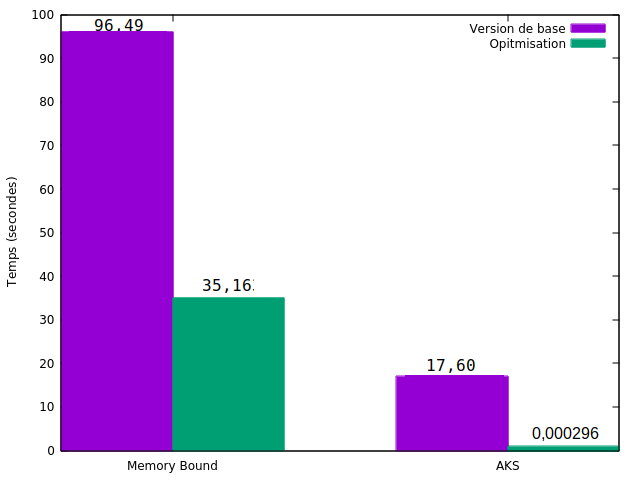
\includegraphics[scale=0.4]{Optimisation.png}\end{center}
		\caption{Comparaison de la version de base avec la version optimisé.}
		\label{fg:fig2}
	\end{figure}	
	\end{frame}
	
	\section{Parallélisation}
	\begin{frame}
	\begin{block}{Outils utilisés}
	\begin{itemize}
		\item OpenMP
		\item MPI (Message Passing Interface)
	\end{itemize}
	\end{block}
	\pause
	\vspace{2.5em}
	\begin{block}{Parallélisation des algorithmes}
	\begin{itemize}
		\item Implémentations non concluantes : AKS, Conjecture, Miller-Rabin, Pocklington 
		\item Implémentation concluante : Memory Bound
	\end{itemize}
	\end{block}
	\end{frame}
	
	
	\begin{frame}	
	\begin{figure}[!ht]	
		\begin{center}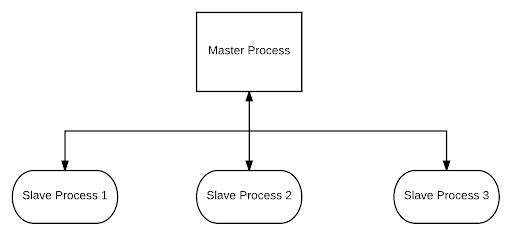
\includegraphics[scale=0.6]{Master1.png}\end{center}
		\caption{Schéma du Modèle du Master-Slave}
		\label{fg:Master}
	\end{figure}
	\end{frame}
	
	\section{Résultats}
	\begin{frame}
		\begin{itemize}
		\item Lancement des tests sur le cluster Poincare de la MDLS. \vspace{2em}
		\item Tests réalisés sur 10 itérations.\vspace{2em}
		\item Lors de la soumission du job Pocklington et AKS n'ont pas pu finir leur exécution avant d'être tué par le supercalculateur.\\
		\end{itemize}
	\end{frame}		
	
	\begin{frame}	
	\begin{figure}[!ht]	
		\begin{center}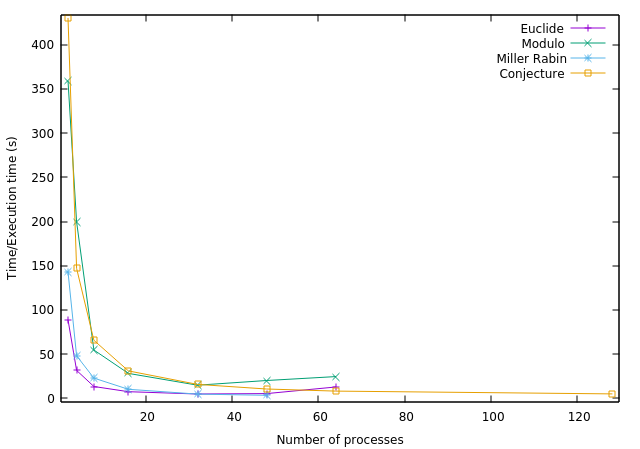
\includegraphics[scale=0.55]{All_1M.png}\end{center}
		\caption{Évolution du temps de calcul pour Conjecture, Miller-Rabin, Euclide et Modulo; Plage [1, 1 000 000]}
		\label{fg:fig1}
	\end{figure}
	\end{frame}

	\begin{frame}
	\begin{figure}[!ht]	
		\begin{center}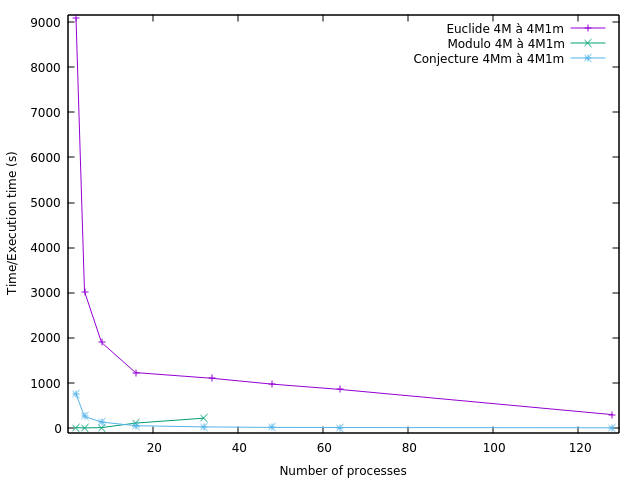
\includegraphics[scale=0.55]{All_4M.png}\end{center}
		\caption{Évolution du temps de calcul pour Conjecture, Euclide et Modulo; Plage [4M, 4M1m]}
		\label{fg:fig2}
	\end{figure}	
	\end{frame}
		
	\begin{frame}
	\begin{figure}[!ht]	
		\begin{center}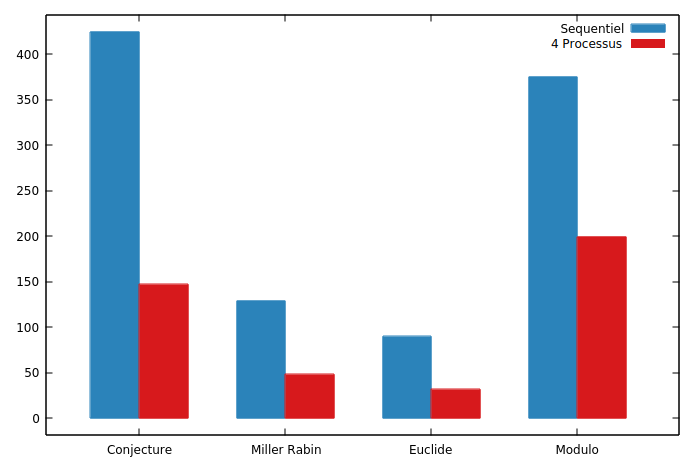
\includegraphics[scale=0.4]{Bar1.png}\end{center}
		\caption{Comparaison Conjecture, Miller-Rabin, Euclide et Modulo avec le séquentiel}
		\label{fg:fig3}
	\end{figure}	
	\end{frame}
		
	\begin{frame}
	\begin{figure}[!ht]	
		\begin{center}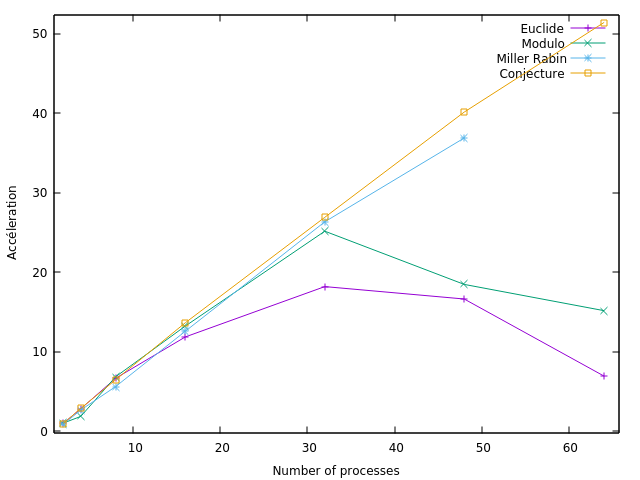
\includegraphics[scale=0.55]{Acc_All_1M_v2.png}\end{center}
		\caption{Évolution de l’accélération en fonction du nombre de processus; Plage [1, 1 000 000].}
		\label{fg:fig4}
	\end{figure}	
	\end{frame}
	
	\begin{frame}
	\begin{figure}[!ht]	
		\begin{center}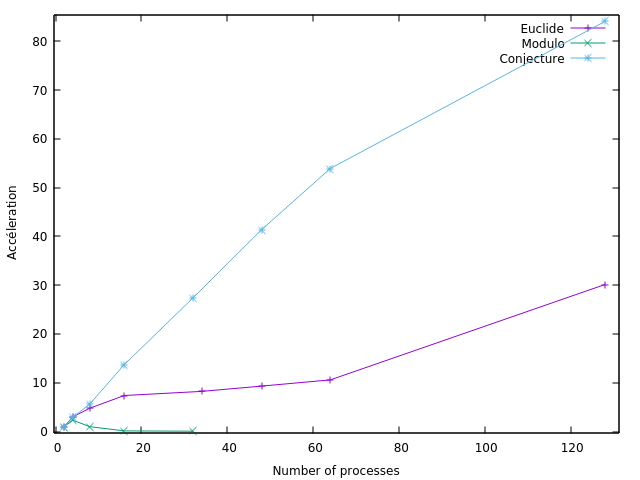
\includegraphics[scale=0.55]{Acc_All_4M.png}\end{center}
		\caption{Évolution de l’accélération en fonction du nombre de processus; Plage [4M, 4M1m].}
		\label{fg:fig4}
	\end{figure}	
	\end{frame}
	
	\begin{frame}
	\footnotesize\begin{longtable}{l l}		
 		\hspace{-2em} 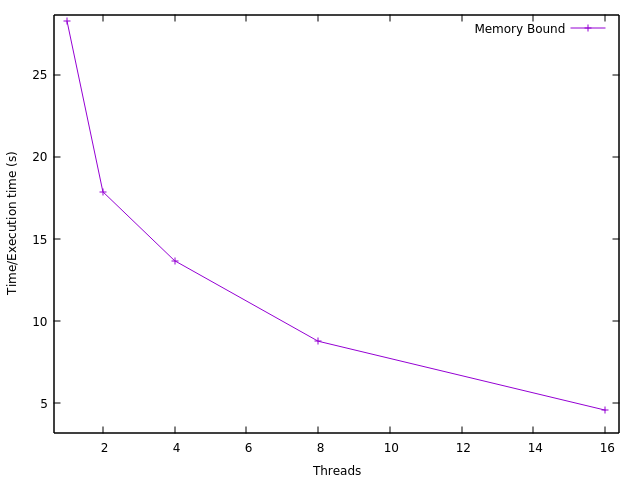
\includegraphics[scale=0.37]{Memory.png}  & \hspace{-1em}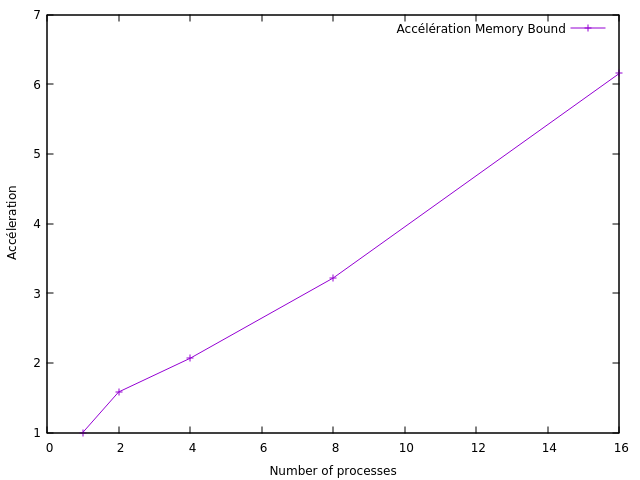
\includegraphics[scale=0.37]{Acc_Memory.png}\\
 			\end{longtable}
		 \color{blue} Figures - \color{black}Évolution du temps de calcul et de l'accélération pour Memory Bound en fonction du nombre de threads. \\
		\end{frame}
	
	\begin{frame}
	\begin{figure}[!ht]	
		\begin{center}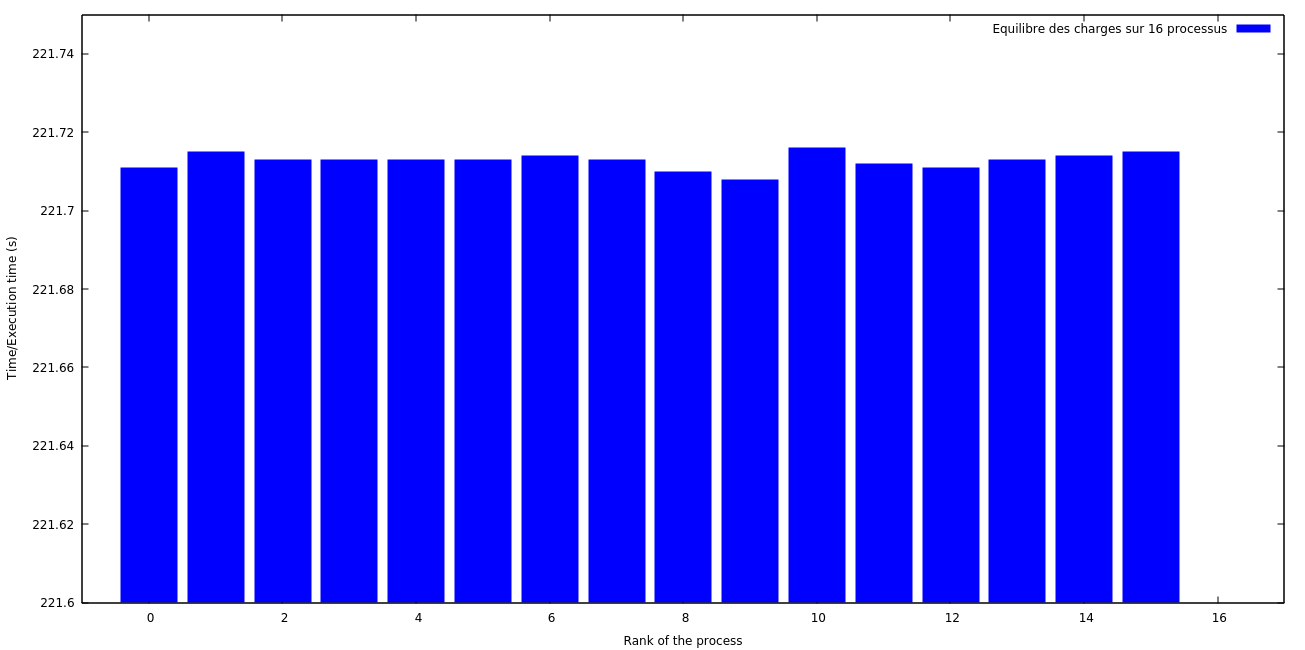
\includegraphics[scale=0.35]{equilibre8.png}\end{center}
		\caption{Exemple d'équilibre des charges obtenu avec 16 processus MPI.}
		\label{fg:fig6}
	\end{figure}	
	\end{frame}
	
	\begin{frame}
	\begin{figure}[!ht]	
		\begin{center}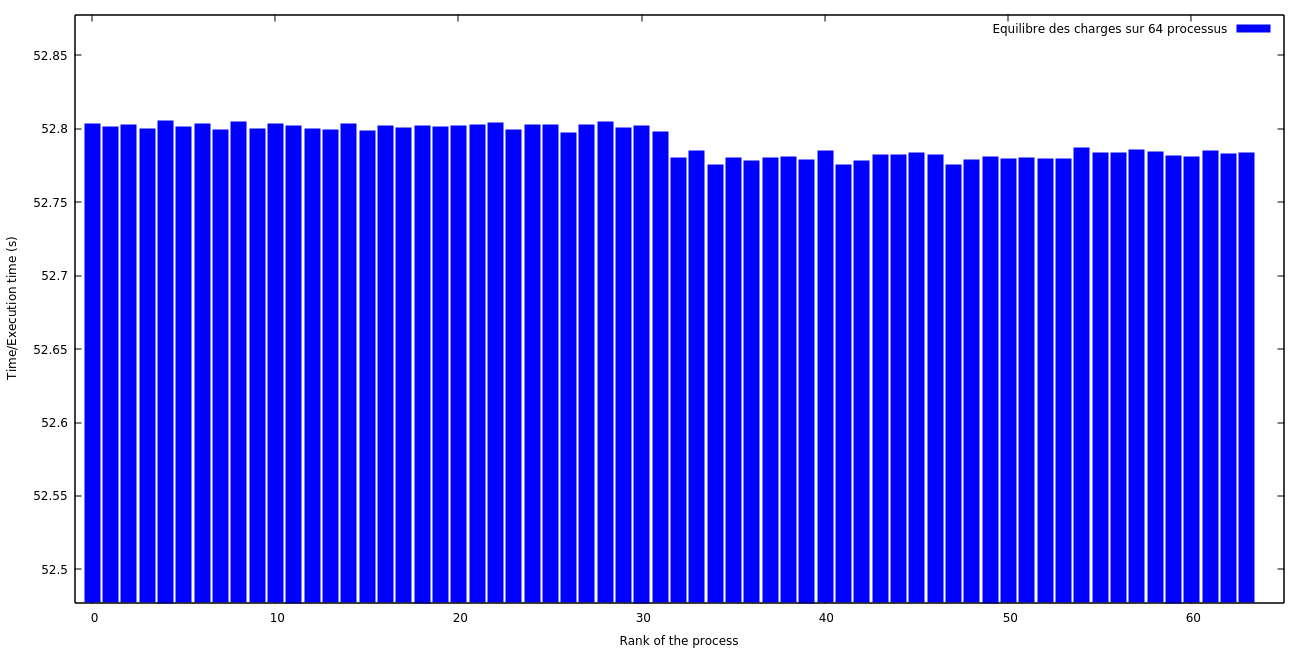
\includegraphics[scale=0.35]{equilibre64.png}\end{center}
		\caption{Exemple d'équilibre des charges obtenu avec 64 processus MPI.}
		\label{fg:fig7}
	\end{figure}	
	\end{frame}
	
	\section{Bilan Technique}
	 
\begin{frame}
\begin{itemize}
\item Une bonne scalabilité forte. \vspace{2em}
\item Un palier max d’accélération.\vspace{2em}
\item Le processus Maître trop chargé en travail.\\
\end{itemize}
\end{frame}

\begin{frame}
\begin{block}{De meilleurs schémas de communications}
\begin{itemize}
\item Augmentation du nombre données à traiter par un esclave à chaque communication du Maître.\vspace{1em}
\item Augmentation du nombre de Maîtres.
\end{itemize}
\end{block}
\end{frame}

\begin{frame}
\begin{figure}[!ht]	
		\begin{center}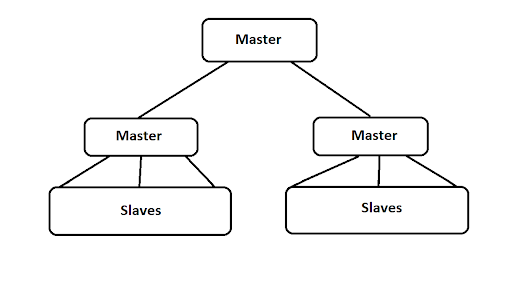
\includegraphics[scale=0.55]{Masters2.png}\end{center}
		\caption{Schéma avec augmentation du nombre de Maître}
		\label{fg:fig12}
	\end{figure}
\end{frame}

\begin{frame}
\begin{block}{Un équilibrage des charges efficace}
\begin{itemize}
\item Des temps de calcul très courts.\vspace{1.5em}
\item Des temps de calcul répartis de manière uniforme. \vspace{1.5em}
\item Des différences finales négligeable entres les processus.\\
\end{itemize}
\end{block}

\end{frame}

\begin{frame}
\begin{itemize}
\item Les tests de primalité sont peu parallélisable. \vspace{2em}
\item Seule l'augmentation du volume de donnée permet de tirer avantage du parallélisme. \vspace{2em}
\end{itemize}
\end{frame}
	
	\section{Problèmes Rencontrés}
	\begin{frame}
\begin{itemize}
\item Utilisation de bibliothèques sur le supercalculateur (NTL, GMP).\vspace{1.5em}
\item Manque de temps. \vspace{1.5em}
\item Dysfonctionnement  du supercalculateur.
\end{itemize}
	\end{frame}
	
	\section{Conclusion}
	\begin{frame}
	\begin{itemize}
\item Résultat final satisfaisant et équilibrage des charges efficace.\vspace{1.5em}
\item Possibilité d’étudier d’autres techniques de parallélisation.\vspace{1.5em}
\item Utilisation d’algorithmes nativement parallèle.
\end{itemize}
	\end{frame}
\end{document}

% Courbes Accélération sur graphes Bar / Calcul de l'accélération
% Préciser à l'oral que les résultats => 10 runs
% XX Graphe pour l'équilibre des charges
% XX Graphes de natures différentes.\\
% XX Accélération ( 5 courbes => 5 accélérations) par rapport au temps séquentiel
% Implem paralléle non-existante (rappel) 
% Parler de l'algorithme de Master-Slave
% Graphe montrant/décrire le Master-Slave( Mettre le graphe après les résultats => transition sur le bilan ?)
% Problèmes avant les Bilan tech/ Ou l'inverse
% Test avec 999995819